%##################################################
% Mock catalogs
%##################################################
\section{Generating mock catalogues}
\bartchapterimage{heic0910i_small.jpg}
\bartthumb{thumbs/heic0910i.png}
\begin{frame}
    \frametitle{Generating mock catalogs}

    \begin{columns}
        \begin{column}{0.5\textwidth}
            % \includegraphics[height=0.8\textheight,angle=-90]{cone.pdf}
        \end{column}
        \begin{column}{0.5\textwidth}
            \begin{alertblock}{Mock catalogs}
                \begin{enumerate}
                    \item<1-> Allow to link redshift space selected groups
                        to real space groups.
                    \item<2-> Constructed from galaxy catalog output of
                        semi-analytical codes applied on Millennium-II run
                        and HOD (halo occupation distribution).
                    \item<3-> Similar to SDSS survey: mask, observational
                        uncertainties\ldots
                \end{enumerate}
            \end{alertblock}
        \end{column}
    \end{columns}
\end{frame}

\begin{frame}
    \begin{tikzpicture}[overlay, remember picture]
        \node[visible on=<1->]
            at ($ (current page.north west) + (3cm, -2cm) $)
            {\includegraphics[width=4cm]{figures/mock.pdf}};
        \node[visible on=<2->]
            at ($ (current page.north west) + (10cm, -2.5cm) $)
            {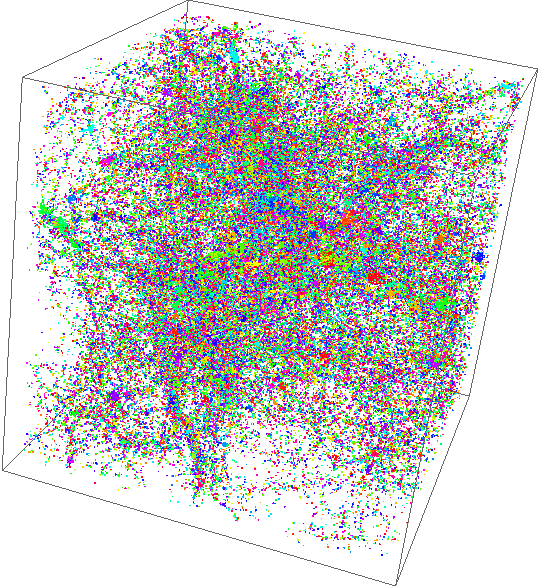
\includegraphics[width=4cm]{figures/cubemock.png}};
        \node[visible on=<3->]
            at ($ (current page.north west) + (10cm, -7cm) $)
            {\includegraphics[width=4cm]{figures/galaxy_mock.jpg}};
        \draw[line width=1pt, visible on=<2->]
            ($ (current page.north west) + (3.3cm, -2.45cm) $) --
            ($ (current page.north west) + (8.2cm, -0.9cm) $);
        \draw[line width=1pt, visible on=<2->]
            ($ (current page.north west) + (3.35cm, -2.75cm) $) --
            ($ (current page.north west) + (8cm, -3.8cm) $);
        \draw[line width=1pt, visible on=<3->]
            ($ (current page.north west) + (9cm, -3cm) $) --
            ($ (current page.north west) + (8cm, -5.45cm) $);
        \draw[line width=1pt, visible on=<3->]
            ($ (current page.north west) + (9cm, -3cm) $) --
            ($ (current page.north west) + (12cm, -5.45cm) $);
    \end{tikzpicture}
    \begin{minipage}[c][0.4\textheight][c]{\linewidth}
    \end{minipage}
    \begin{minipage}[c][0.6\textheight][c]{0.5\linewidth}
        \begin{block}{HOD or SAM}

        \end{block}
    \end{minipage}
\end{frame}

\begin{frame}
    \begin{tikzpicture}[
        mindmap,
        concept color=blue!60!white,
        text=white,
    ]
        \node[concept] (initial){%
            \begin{tikzpicture}[scale=0.5]
                \draw[
                    domain=0:6,
                    smooth,
                    variable=\x,
                    blue,
                    samples=500,
                    line width=1pt,
                    label={0.5}{$\lambda_0$},
                ]
                plot ({\x}, {sin(10*\x r)});
            \end{tikzpicture}%
        }
        child[grow=right, visible on=<2->, concept
            color=blue!50!red!60!white, level distance=4.5cm] {%
                node[concept] (cosmo){%
                
\begin{tikzpicture}[scale=0.3]
                    \draw[
                        domain=0:6,
                        smooth,
                        variable=\x,
                        blue!50!red,
                        samples=500,
                        line width=1pt,
                    ]
                        plot ({\x}, {sin(5*\x r)});
                \end{tikzpicture}
            }
            child[visible on=<3->, concept color=red!60!white] {%
                node[concept] (peculiar){%
                    
\begin{tikzpicture}[scale=0.2]
                        \draw[
                            domain=0:6,
                            smooth,
                            variable=\x,
                            red,
                            samples=500,
                            line width=1pt,
                        ]
                            plot ({\x}, {sin(\x r)});
                    \end{tikzpicture}
                }
            }
        };
        \node[below, text=blue, visible on=<1->] at (initial)
            {Emitted\\$\lambda_0$};
        \node[below, text=blue!50!red, visible on=<2->] at (cosmo) {%
            Expansion\\$\left(1+z_{\cos}\right) \lambda_0$
        };
        \node[below, text=red, visible on=<3->] at (peculiar) {%
            Peculiar velocity\\
            $\left(1+z_\mathrm{pec}\right)\left(1+z_{\cos}\right) \lambda_0$
        };
    \end{tikzpicture}
\end{frame}
